\documentclass[11pt]{article}
\usepackage{graphicx}
\usepackage{hyperref}
\usepackage[dvipsnames, svgnames, x11names, hyperref]{xcolor}
\hypersetup{
	colorlinks,
	citecolor=Violet,
	linkcolor=Red,
	urlcolor=Blue}
\usepackage{natbib}
\usepackage{amsmath}
\usepackage{siunitx}

\setlength{\textwidth}{6.5in}
\setlength{\headheight}{0in}
\setlength{\textheight}{8.0in}
\setlength{\hoffset}{0in}
\setlength{\voffset}{0in}
\setlength{\oddsidemargin}{0in}
\setlength{\evensidemargin}{0in}


\title{Homework 8 Solution}

\author{Nana Ama Nyamekye Darpaah}

\begin{document}
	
	\maketitle
	\section{Question 1}
	The probability can be expressed as 
	
	\begin{equation}
		p(x) = \frac{1}{1 + \exp[-(\beta_{0}+\beta_{1}x)]}
	\end{equation}

	Rearranging to prevent underflows, we get
	\begin{equation}
		likelihood = \sum(\log(1-p)+y\log(\frac{p}{1-p}))
	\end{equation}
	
	where p is the logistic function of the probability.
	
	Scipy.optimize was used to calculate the minimum of the likelihood.
	
	The minimum was found to be at 34.725622 years after 12 iterations. The values of $\beta_{0}$ and $\beta_{1}$ were calculated to be -5.62023183 and 0.10956338. The covariance matrix, which is represented as the Hessian inverse was found to be \\
	
$	\begin{bmatrix}
		1.40236908e-4 & -3.46818473e-5\\
		-3.46818473e-5 & 4.81700786e-5
	\end{bmatrix}$
\\
The error can be expressed as the square root of the diagonal entries in the covariance matrix. Hence, the error is
	$\sqrt{Hess[0,0]} = \sqrt{1.40236908e-4} = 0.7206169643856918$
	
	The plot of both the original response, given as 1(0) for response yes(no), and the logistic model is seen in Figure \ref{fig:likelihood}
	
	\begin{figure}[!htb]\begin{center} 
			\vspace{12pt}
			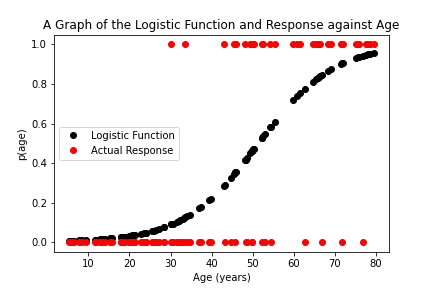
\includegraphics[width=0.7\textwidth]{Likelihood.png}
			\caption{A plot of response and likelihood against age}
			\label{fig:likelihood} 
		\end{center}
	\end{figure}
	
	
	
	
	
	
	\section{Question 2}
	A plot of the data contained in the piano dataset is as shown in Figure \ref{fig:piano}.
	Fast Fourier Transform (FFT) was applied by means of the numpy.fft.rfft module on both the trumpet and piano datasets. A log graph was plotted for better scaling as seen in Figure \ref{fig:piano_trumpet}.
	
	\begin{figure}[!htb]\begin{center} 
			\vspace{12pt}
			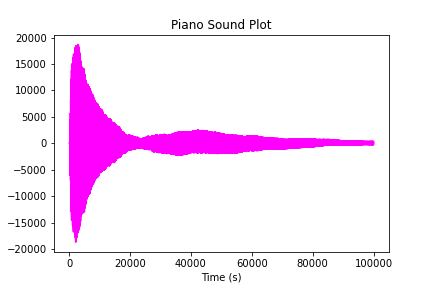
\includegraphics[width=0.7\textwidth]{piano.png}
			\caption{A plot of a piano signal}
			\label{fig:piano} 
		\end{center}
	\end{figure}
	
	\begin{figure}[!htb]\begin{center} 
			\vspace{12pt}
			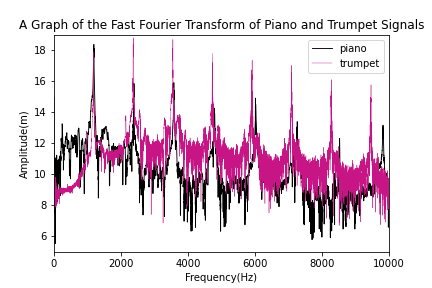
\includegraphics[width=0.7\textwidth]{piano_vs_trumpet_fft.png}
			\caption{A plot of the piano and trumpet signal after FFT}
			\label{fig:piano_trumpet} 
		\end{center}
	\end{figure}
	
	\section{Question 3}
	Dow data was obtained and the FFT was applied. Copies of the data after the transform were made and all but the first 10 percent of the values(dow\_10) were set to zero. Also, the first 2 percent of values(dow\_2) were maintained and the rest, set to zero. An inverse FFT was then applied and the results, plotted.
	The graph containing the plots of all three data are seen in Figure \ref{fig:dows}
	\begin{figure}[!htb]\begin{center} 
			\vspace{12pt}
			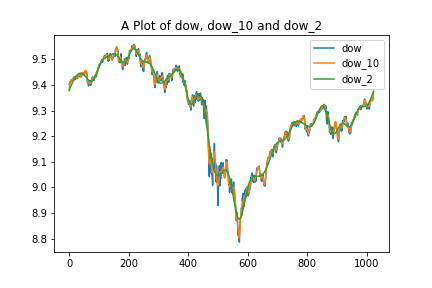
\includegraphics[width=0.7\textwidth]{dows.png}
			\label{fig:dows} 
		\end{center}
	\end{figure}
	
	
	A zoomed in image of the plot gives a clearer view of the nature of each plot. From Figure \ref{fig:dow_zoomed}, it can be seen that the plot of dow\_10 somewhat follows the general trend of the original transformed data. The plot of dow\_2 is much smoother and keeps barely any of the original data's information.  
	\begin{figure}[!htb]\begin{center} 
		\vspace{12pt}
		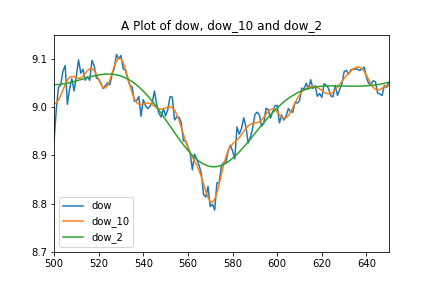
\includegraphics[width=0.9\textwidth]{dow_zoomed.png}
		\label{fig:dow_zoomed} 
	\end{center}
	\end{figure}
			
\end{document}